\section{Conclusion and Future Work}
In the pursuit of human happiness and well-being, it is critical to assist individuals in being more honest. This goal has aided in the development of a new type of assistive technology capable of anonymously linking people with mental health specialists in order to overcome the limitations of anonymity and security in videoconferencing therapy, as well as the lack of expressiveness in text/phone therapy. 

One of the main contributions of our work involves the use and development of new capabilities with ultra-realistic virtual human avatars known as Metahumans. Despite the fact that other researchers have addressed problems similar to ours \cite{LU21, ZAL18, GRA07, LUC14, ROT19, KAN16, KAN10A, BAC19}, our work is essential because the VA used in this experiment are new and unexplored. Furthermore, they demonstrate more realistic human features than other works, meaning that similar works' findings cannot be considered relevant because the conditions are different.

Our primary study assessed users' empathy with metahumans in order to determine whether these virtual avatars were able to convey the same emotional depth as a real person (\textbf{RQ\textsubscript{1}}). To find out if our stimulus had an impact, we conducted a between-subjects experiment with 48 participants to measure their CE and AE. The findings of this study were a first step toward a better understanding of the potential use of ultra-realistic virtual human avatars in videoconference therapy. They also revealed that the virtual avatar's lack of hand movement constrained their capacity to express themselves, giving the impression that they were acting like puppets or in an unnatural way. This particular result led us to wonder whether or not the addition of hand tracking would aid improve interactants' verbal self-disclosure (\textbf{RQ\textsubscript{2}}).

According to many studies \cite{ARJ20, WAX97, REI22}, hand gestures, together with facial expressions and spoken words, play a significant part in transmitting our emotions. As a result, incorporating hand tracking into our prototype is a critical step toward our aim of deeper emotional detection. Because, aside from facial expressions and body posture, the most crucial nonverbal clues for distinguishing specific states in others are hands \cite{WAX97, REI22}.

Through controlled prototype testing, as well as a questionnaire, our second study investigated the viability of our work and tested users' acceptance of the application as well as users' OPD. Despite the fact that not all of our hypotheses were accepted, through the study's findings, we were able to acknowledge the potential of our work and analyze what could be lacking and improved to make our work truly useful and easy to use. Furthermore, we attempted to determine whether virtual avatars may improve users' verbal self-disclosure (\textbf{RQ\textsubscript{2}}), but we were unable to confirm it since we could not establish a relationship between the users' perceived anonymity and online public disclosure.

Overall, our research improved our comprehension of the prospective use of ultra-realistic virtual human avatars in videoconferencing therapy, i.e., both studies helped us understand how vital facial and body expressions are and how problematic their absence is in communicating with others \cite{KNA13}. It was, however, impossible to discover a relation between users' perceived anonymity and online public disclosure. This correlation was fundamental for our work since it allowed us to determine whether the role of virtual avatars was beneficial to users.

Despite our findings being relatively good, plenty of improvements that could be done in order to achieve better results were postponed due to time constraints. In the following sections, we provide some of the outstanding parts of this work that deserve additional development and investigation:

\subsection{Custom Metahuman Parameters}
One of the most important things for the anonymous face tracking panda application to work is obtaining a facial mesh, which is a 3D representation of a face that allows us to provide data to express ourselves through the metahuman's face. 

Although the current prototype performs the most of the captured facial expressions, a minor issue with the metahumans' lip position was discovered during the second experiment. As a result, since each user has a unique facial mesh that is never exactly the same as someone else's, the modification performed in Chapter III (Figure \ref{fig:blueprintAnimation}) does not permit covering all application users. 

This issue could be resolved by including a calibration option that would enable the definition of a constant that would address the issue of lip position in the metahuman in accordance with each individual's lip position. 

\subsection{Custom Metahuman Upload}
In addition to the four existing metahumans (Figure \ref{fig:metahumans}), it would be intriguing to add the ability to import customized metahumans. This additional feature would allow users to engage with the anomynous panda application more effectively, potentially making them feel more at ease with their new physical appearance. Furthermore, this could boost people's willingness to expose their circumstances and be themselves without fear of being criticized by others.

\subsection{In-app Videoconference}
Because our primary goal is to connect mental therapists with patients, videoconferencing is a vital step in this initiative. Although our work can already be used as a virtual camera, it is critical to make this feature more practical and independent of other external programs (see Figures \ref{fig:prototype} and \ref{fig:obs}), such as OBS Studio, because not all users have medium/advanced computer skills to understand what is required. One solution could be to make our work available remotely using \cite{PIXUE} (similar to Figure \ref{fig:cloud}), with only the patient providing inputs to the metahuman such as face and hand tracking information and both patient and therapist on an embedded videoconference. 

\begin{figure}[!htb]
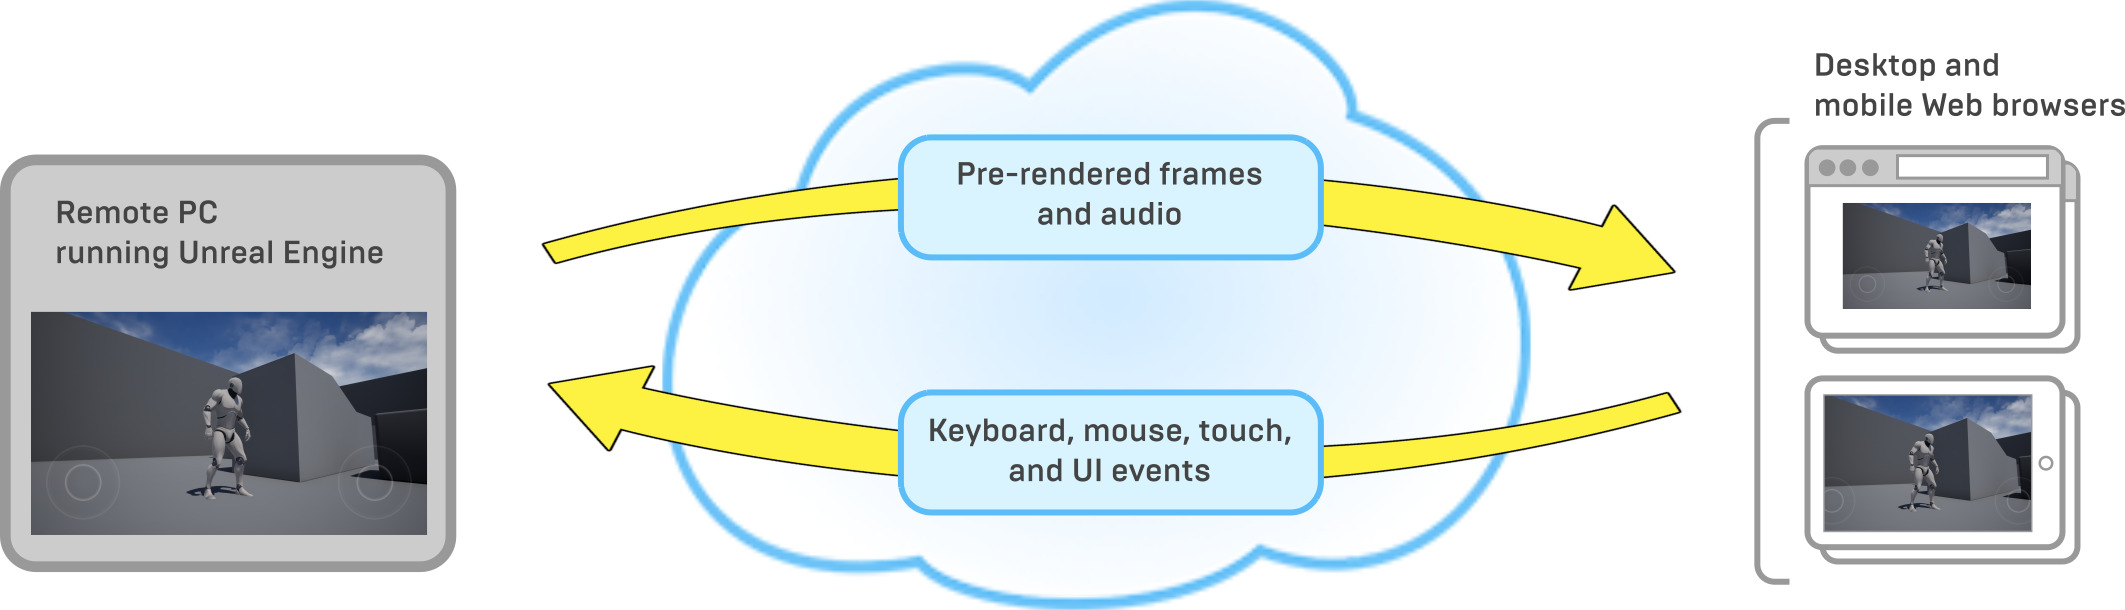
\includegraphics[width=\textwidth]{figures/cloud-simplified.png}
\centering
\caption{UE application working remotely \cite{PIXUE}}
\label{fig:cloud}
\end{figure}

\subsection{Voice Anonymization}
The user's voice being made anonymous is another crucial feature to include. This feature, in addition to increasing anonymity, will allow the user to feel more at ease during their online session of mental therapy, increasing willingness to expose their circumstances and be themselves without fear of others recognizing their voice. However, a simple pitch change is insufficient to mask a voice, as an entity could simply pitch the audio back to recover the original audio. This means that additional research may be required in order to find a solution.

\subsection{Correlation between PA and OPD}
As previously said, additional research into the relationship between users' perceived anonymity and online public disclosure is important since it may indicate how our metahumans play the role of anonymity when used in videoconferencing. The addition of customized metahumans, as well as the integration of voice anonymization, could improve this relationship, but everything inevitably depends on the user and how they perceive the potential and value of our work.

% \subsection{UX/UI Improvements}
% In addition to the features mentioned above, some enhancements to the application's UX/UI would be recommended. One of the most significant improvements would be the addition of simple nudges that would allow the user to be reminded of certain actions in an unobtrusive manner, such as remembering that they have hand tracking available or that they need to establish a direct connection between the iOS device and Anonymous Panda for face tracking to work.

\subsection{Influence on Mental Health Therapy}
Finally, a new study could help understand Anonymous Panda’s influence in mental health therapies. It would also be interesting to learn what it would be like for a therapist to read facial/body expressions and feelings through our metahumans, and whether they would be able to identify all of the information needed during a mental health therapy, among other things, and then use those results to improve our work.

\subsection{The Dark Side of Anonymity}
Anonymity is frequently used to protect people's privacy, such as when reporting the results of a scientific study or describing individual cases. Many countries even have laws that protect anonymity under certain conditions. For example, a person may consult a priest, doctor, or lawyer and reveal sensitive personal information. However, anonymity is not always guaranteed in confessional situations. If a client informs a lawyer that he intends to commit a serious crime, some countries permit or even require the lawyer to notify the police. The choice is difficult because people who tell a priest or a psychologist that they intend to commit a serious crime frequently do so to express their feelings rather than their true intention. To summarize, anonymity can be used for both good and bad. In many cases, anonymity is desirable for one person but undesirable for another. However, there has always been a dark side to anonymity.

Anonymity can be used to protect a criminal who is committing a variety of crimes such as slander, child pornography distribution, illegal threats, racial agitation, fraud, and intentional damage (e.g. distribution of computer viruses). The precise list of illegal acts varies by country, but the majority of countries have numerous laws prohibiting various informational acts ranging from high treason to swindling. Anonymity can also be used to locate contacts for illegal activities, such as a swindler looking for victims. Even when it is not illegal, communicating anonymously can be offensive or disruptive. Some people, for example, use anonymity to make derogatory remarks about others.

In conclusion, the border between illegal and legal is not always clear, as it varies depending on the laws of each country. And since we can not define this barrier, there is not a way for us to limit the use of our application.

\subsection{Prospective Users}
Although the Anonymous Panda app was firstly envisioned to be used by a more generalized public, vulnerable or at-risk populations might benefit from such a system even further. They include, but are not limited to, people who are stigmatized or negatively affected by their sexual orientation or gender identity, allowing them to talk to health professionals or publicly express themselves freely without suffering additional discrimination---which is central to one's mental wellbeing. The same could be the case for people struggling with different physical disabilities and mental health conditions (e.g. body dysmorphia). 

Furthermore, victims of abuse, Alcoholics Anonymous, and army veterans might also benefit from the added privacy protection systems like the Anonymous Panda creates. Such computer-mediated mental health platforms might also be implemented in business settings, where mental health monitoring systems raises serious privacy concerns related to employees' anonymity, for example, or how employers may handle or possibly misuse workers' personal data \cite{XUE19}.
